

\actTitle{Worksheet 4.7B}

\noindent \textbf{Instructions:}  Work together in groups of  3 or 4 to complete the following problems.\\

\begin{enumerate}

\item Find the exact values of the following.
\begin{enumerate}

\item $\cos \left( \tan^{-1}\left(\frac{\sqrt{3}}{3}\right)\right)$

\vfill
\item $\tan \left( \sin^{-1}\left(-\frac{2}{3}\right)\right)$


\vfill

\item $\sin \left( \cos^{-1}\left(\frac{3}{4}\right)\right)$
\vfill

\item $\sec \left( \tan^{-1}\left(\frac{4}{3}\right)\right)$
\vfill

\end{enumerate}



\clearpage
\item Write the expression as an \textbf{algebraic} expression.
  (There should be no trig functions in your answers.)

\begin{enumerate}

\item $\displaystyle \sin \left( \cos^{-1}\left(\frac{\sqrt{x^2-25}}{x}\right)\right)$ for $x>5$

\vfill

\item $\displaystyle \tan \left( \cos^{-1}\left(\frac{3}{x}\right)\right)$ for $x>3$
\vfill

\item $\displaystyle \sin \left( \tan^{-1}\left(x\right)\right)$ for $x>0$
\vfill


\end{enumerate}


\clearpage

\item A toy car rolls down a straight ramp. The length of the ramp is
  30m and the amount of altitude lost is 8m, what is the angle of
  incline?  Round to the nearest tenth of a \textbf{degree}.

  \vfill

\item A video camera located at ground level follows the liftoff of a
  rocket.  Suppose that the camera is 1500 m from the launch pad.
\begin{enumerate}
\item Determine the angle of elevation $\theta$ from the camera to the
  rocket as a function of the rocket's height, $h$.
  
  \vfill
  
\item Use a calculator to approximate the angle of elevation to the
  nearest tenth of a degree when the rocket's height is 1000 m, 2000
  m, and 5000 m. What are the range of possible values of the angle of
  elevation?
  
  \vfill
\end{enumerate}

\clearpage
\item Determine the value of $\theta$ associated with the coordinate
      in the figure below. (Numerical answers should be to within 2
      decimal digits.)

      \begin{tikzpicture}[y=0.4cm, x=0.4cm,font=\sffamily]
        \draw[thick,black] (-5,0) -- (5,0) node[anchor=west] {$x$};
        \draw[thick,black] (0,-5) -- (0,5) node[anchor=south] {$y$};
        \draw[thin,black] (0,0) -- (-3.5,-5);
        \draw[thin,black] (0,0.6) arc (90:235:0.6) node[pos=0.5,anchor=south east] {$\theta$};
        \node[black,anchor=east] at (-3.5,-5) {$(-3.5,-5)$};
        \draw[black,fill=black] (-3.5,-5) circle (0.5ex);
      \end{tikzpicture}

\item Determine the \textbf{exact} values of each of the
  expressions below. (Do not use a value from a calculator but derive the true value.)
  \begin{enumerate}


  \item
    ${\displaystyle \cos\left(\pi -  \arcsin\left(\frac{3}{5}\right) \right) }$ 
    \vfill
    
   \item
    ${\displaystyle \cos\left(\pi + \arcsin\left(\frac{3}{5}\right) \right) }$ 
    \vfill
    
      \item
    ${\displaystyle \cos\left(2\pi - \arcsin\left(\frac{3}{5}\right) \right) }$ 
    \vfill   
    


  \end{enumerate}

\end{enumerate}

\hwTitle{Section 4.7B}

\begin{enumerate}
\item Determine the domain of each function below.
  \begin{enumerate}
  \item ${\displaystyle \arccos\left(\frac{x+1}{5}\right) }$
  \item ${\displaystyle \arcsin\left(e^x\right) + \frac{1}{x}}$
  \item ${\displaystyle \sin^{-1}\left( \ln(x) \right) }$
  \item ${\displaystyle \cos^{-1}\left( \frac{5}{x} \right)  }$
  \end{enumerate}
\item A surveyor will use the angle of elevation to determine the
  height of a building. The height is estimated to be between 45m and
  50m tall. The surveyor has limited room to work and will have to be
  a distance between 70m and 85m from the base of the building. If you
  only have two locations to use which ones should you use to
  approximate the extremes in the angle of elevation? What is the
  possible range of values for the angle of elevation?
\item A weather radar system can discern clouds whose angle of
  resolution is an angle $\theta$. The smallest cloud that can be
  resolved at 30,000m is 70m wide. What is the angle of resolution for
  the system? What is the smallest cloud that can be detected that is
  40,000m away?

  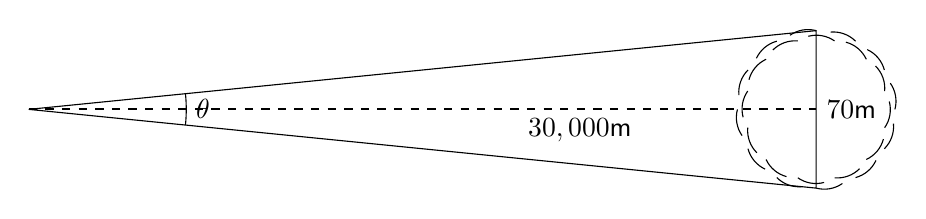
\begin{tikzpicture}[y=1.0cm, x=1.0cm,font=\sffamily]

    \foreach \x in {0,1,2,...,11} %{30,120,210,300}
    {
      \draw[] (10,0)++(30*\x:1) arc (30*\x-15:30*\x+35:0.4);
      \draw[] (10,0)++(30*\x+15:.9) arc (30*\x-5:30*\x+45:0.4);
    }
    \draw[thick,black,dashed] (0,0) -- (10,0) node[anchor=west] {$70$m};
    \node[anchor=north] at (7,0) {$30,000$m};
    \draw[black] (0,0) -- (10,1) -- (10,-1) -- cycle;

    \draw[thin,black] (-5.7:2) arc (-5.7:5.7:2) node[pos=0.5,anchor=west] {$\theta$};
  \end{tikzpicture}

\item A helicopter will take off from a landing pad, and it will rise
  straight up at a constant speed of three meters per second. A camera
  will be placed 400 meters away from the pad and will be aimed at the
  helicopter. What should the angle of elevation of the camera be 30
  seconds after the helicopter takes off?

\item A Ferris wheel has a radius of 25 meters, and the center of the
  wheel is 28 meters off the ground. At the initial time a seat is at
  the bottom of the wheel. At what time will the seat first be 12
  meters above the ground? At what time will the seat be 12 meters
  above the ground for the second time?

\end{enumerate}
